\documentclass[tikz, border=5pt]{standalone}
\usepackage{tikz}
\usetikzlibrary{angles, quotes} % 用于绘制角度标记

\begin{document}
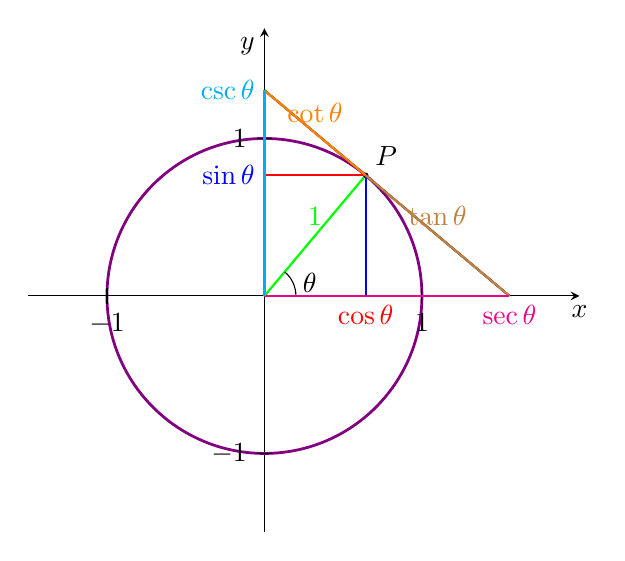
\begin{tikzpicture}[>=stealth, scale=2] % 缩放使图形更清晰

    % 绘制坐标轴
    \draw[->] (-1.5,0) -- (2,0) node[below] {$x$};
    \draw[->] (0,-1.5) -- (0,1.7) node[below left] {$y$};

    % 绘制单位圆(紫色)
    \draw[violet, line width=1pt] (0,0) circle (1);

    % 标记坐标轴刻度
    \foreach \x in {-1,1} \draw (\x,0.05) -- (\x,-0.05) node[below] {$\x$};
    \foreach \y in {-1,1} \draw (0.05,\y) -- (-0.05,\y) node[left] {$\y$};

    % 定义角度θ(示例取50度,可修改为任意角度)
%    \def\theta{50}
%    \pgfmathsetmacro{\sintheta}{sin(\theta)} % sinθ 正弦sine
%    \pgfmathsetmacro{\costheta}{cos(\theta)} % cosθ 余弦cosine
%    \pgfmathsetmacro{\tantheta}{tan(\theta)} % tanθ 正切tangent
%    \pgfmathsetmacro{\sectheta}{1/cos(\theta)} % secθ=1/cosθ 正割secant
%    \pgfmathsetmacro{\csctheta}{1/sin(\theta)} % cscθ=1/sinθ 余割cosecant
%    \pgfmathsetmacro{\cottheta}{1/tan(\theta)} % cotθ=1/tanθ 余切cotangent
    
%     \def\theta{50} % 取消定义角度,直接输入,后续theta可显示符号θ
    \pgfmathsetmacro{\sintheta}{sin(50)} % sinθ
    \pgfmathsetmacro{\costheta}{cos(50)} % cosθ
    \pgfmathsetmacro{\tantheta}{tan(50)} % tanθ
    
    \pgfmathsetmacro{\sectheta}{1/cos(50)} % secθ=1/cosθ
    \pgfmathsetmacro{\csctheta}{1/sin(50)} % cscθ=1/sinθ
    \pgfmathsetmacro{\cottheta}{1/tan(50)} % cotθ=1/tanθ
    

    % 绘制角度θ的射线(绿色)
    \draw[thick] (0,\csctheta) -- (\sectheta,0); % 坐标轴上的交点
    \draw[green, thick] (0,0) -- (\costheta,\sintheta) node[midway, above] {1};

    % 画弧线,标记角度θ
    \draw (0.2,0) arc (0:50:0.2) node[midway, right] {$\theta$};

    % 绘制单位圆上的点与投影(红red、粉pink、蓝blue、绿green、黄yellow、橙orange、紫purple、白white、黑black)
    \fill (\costheta,\sintheta) circle (0.5pt) node[above right] {$P$}; % 单位圆上的交点
    
    \draw[blue, thick] (\costheta,0) -- (\costheta,\sintheta); % sin(θ)竖直线
    \node[red, below] at (\costheta,0) {$\cos\theta$};
    
    \draw[red, thick] (0,\sintheta) -- (\costheta,\sintheta); % cos(θ)水平线(sin(θ)的x投影)
    \node[blue, left] at (0,\sintheta) {$\sin\theta$};
    
    \draw[brown, thick] (\sectheta,0) -- (\costheta,\sintheta) node[midway, above] {$\tan\theta$}; % tan(θ)长度
    
    \draw[orange, thick] (0,\csctheta) -- (\costheta,\sintheta) node[midway, above] {$\cot\theta$}; % cot(θ)长度
    
    \draw[magenta, thick] (0,0) -- (\sectheta,0) ; % secθ长度 正割
    \node[magenta, below] at (\sectheta,0) {$\sec\theta$};
    
    \draw[cyan, thick] (0,0) -- (0,\csctheta) ; % cscθ长度
    \node[cyan, left] at (0,\csctheta) {$\csc\theta$};

\end{tikzpicture}
\end{document}
